
\subsection{Answers}
\begin{table}[htb]%
\begin{center}%
\caption{Q28: Do you think the MPI standard should maintain backward compatibility?}%
\label{tab:Q28-ans}%
\begin{tabular}{l|l|r}%
\hline%
Choice & Abbrv. & \# Answers \\%
\hline%
{\small Yes, compatibility is very important for me.} & Very important & 304 (36.8\%) \\%
API should be clearly versioned. & Versioned API & 186 (22.5\%) \\%
{\small I prefer to have new API for better perf$\cdots$} & New API for performance & 127 (15.4\%) \\%
{\small I prefer to have new API which is simple$\cdots$} & New API for easier-to-use & 124 (15.0\%) \\%
I do not know or I do not care. & Do not know/care & 74 (9.0\%) \\%
other & - & 11 (1.3\%) \\%
\hline%
\multicolumn{2}{c}{total} & 826 \\%
\hline%
\end{tabular}%
\end{center}%
\end{table}%


This question is about backward compatibility of the MPI API. More than one
third of the users think that this is important that the MPI API keep backward
compatibility from version to version. The question of the evolution of the
standard for easier use or better performance is, in total,  supported by 30\%
of the users. Almost 9\% do not care and the middle ground consisting of having
a versionned API is supported by 23\% of the users. There is no real discrepancy in
terms of region for this question. 

Conversely speaking, 60\% users may accept new, not backward-compatible API.

\subsection{List of other answers}
\begin{itemize}
\item Europe:France: I think the MPI standard should evolve more quickly, and drop backward compatibility when necessary
\item Europe:Germany: Would be nice, but sometimes one has to move forward.
\item Europe:Germany: compatibility for a typical "PhD completion" window is a must
\item Europe:Germany: compatibility is important, but should be sacrificed if necessary to implement important changes, e.g. to support 64-bit ints for message lengths
\item Europe:UK: Both "I prefer to have new API for better performance" and "API should be clearly versioned"
\item Europe:UK: The weasel response - I want the code I use to be backward compatible, but don't mind if other bits break!
\item Europe:others: Comnpatibility is important, but it is okay to delegate old API to a different module/header
\item Europe:others: Compatibility is helpful because of the large codebase.
\item Europe:others: Hard question to answer either or on. It should be clearly versioned, mainly backward compatible unless impossible by important future performance and/or interop reasons. Clear enough?;-)
\item Europe:others: The gist of this survey is that you want to know if the API should be changed. The existing API is a good fit for existing functionality: it is a bit clunky, but the standard is clear, and it is easy to wrap in clean C++. The main problem with the API is that only a small part of the API is effiniently/correctly implemented on many implementations.
\item Russia: I prefer to have new API for better performance. But now I have small parallel programmes.

\end{itemize}

\begin{figure}[htb]
\begin{center}
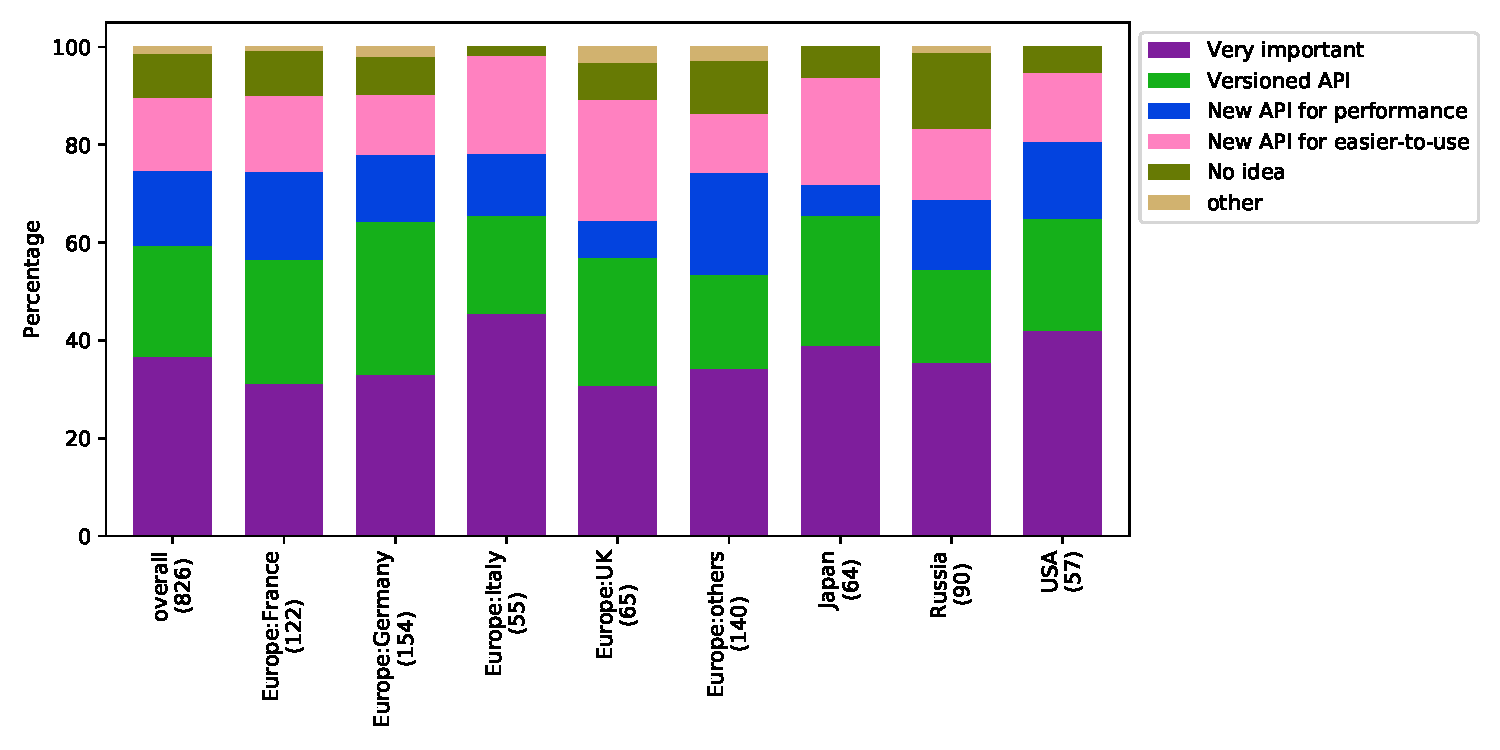
\includegraphics[width=10cm]{../pdfs/Q28.pdf}
\caption{Simple analysis: Q28}
\label{fig:Q28}
\end{center}
\end{figure}
